\documentclass[9pt]{beamer}

\usepackage{beamerpreamble}
\usepackage[swedish]{babel}
\usepackage{minted}
\usepackage{comment}
\usemintedstyle{vs}
\usepackage{xcolor}
\usepackage{tikz}
\usepackage{textgreek}
\usepackage{dirtytalk}
\usepackage{xcolor}

\renewcommand{\ttdefault}{cmtt}

\newcommand*\mean[1]{\bar{#1}}

\title{Datalaboration - Förberedande tutorial}
\author[benjamin.eriksson@physics.uu.se]{Benjamin Eriksson  \\ \tiny{med inspiration från} \\ \scriptsize{Slides av M. Isacson, M. Ellert, M. Olvegård, och B. Lindgren}}
\institute[Uppsala universitet]{{\small Avdelningen för tillämpad kärnfysik \\ Institutionen för fysik och astronomi} \\ \uulogo}
\date{{\small Reviderad}\\ \today}

\begin{document}

    \begin{frame}{Minstakvadratmetoden}
        Efter denna modul ska du kunna
        \begin{itemize}
            \item bestämma lutning och skärningspunkt utifrån minstakvadratmetoden
            \item bestämma osäkerheterna i lutningen och skärningspunkten
        \end{itemize}
    \end{frame}

    \begin{frame}
        Vi är oftast intresserade av \emph{funktionella samband} mellan två
        eller flera storheter. 

        \begin{itemize}
            \item Position $s$ som beror av en tid $t$
            \item Ström $I$ beroende av en pålagd spänning $V$
            \item Periodtid $T$ beroende av pendelarm $L$
            \item \ldots
            \item Storhet $y$ beroende av $x$, alltså $y(x)$
        \end{itemize}

        Genom att variera $x$ och mäta $y$ fås två mätserier $\{x_i\}_1^n$ och
        $\{y_i\}_1^n$, alternativ en mätserie av paren $\{x_i,y_i\}_1^n$.

        \vfill
        \begin{columns}
            \column{.5\textwidth}
            Hur finner vi sambandet $y=f(x)$ med hjälp av dessa mätningar?
            \column{.5\textwidth}
            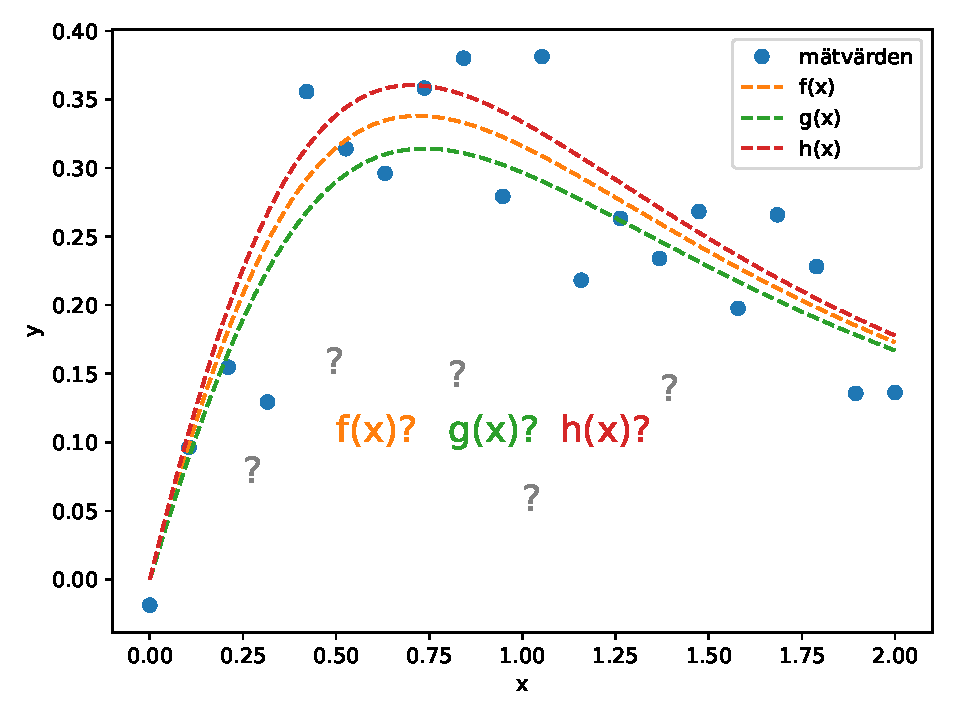
\includegraphics[width=\textwidth]{anpassning0.pdf}
        \end{columns}

    \end{frame}

    \begin{frame}
        Sambandet $f$ kan t.ex. vara en teoretisk modell beroende på ett antal parameterar $a_j$, dvs
        \begin{equation*}
            y = f(x,a_1, a_2, \ldots, a_m) \quad \left[\text{t.ex.} \ y = a_1 + a_2x + a_3x^2 \right]
        \end{equation*}

        \vfill

        \begin{columns}
            \column{.5\textwidth}
            Hur bra beskriver $f$ vår mätdata $\{x_i,y_i\}$? Bilda kvadratsumman $S$:
            \begin{equation*}
                S = \sum_i\left(y_i - f(x_i,a_1,\ldots,a_m)\right)^2
            \end{equation*}
            $\rightarrow$ Ju mindre skillnad mellan $y_i$ och $f(x_i)$ desto mindre blir $S$.

            \column{.5\textwidth}
            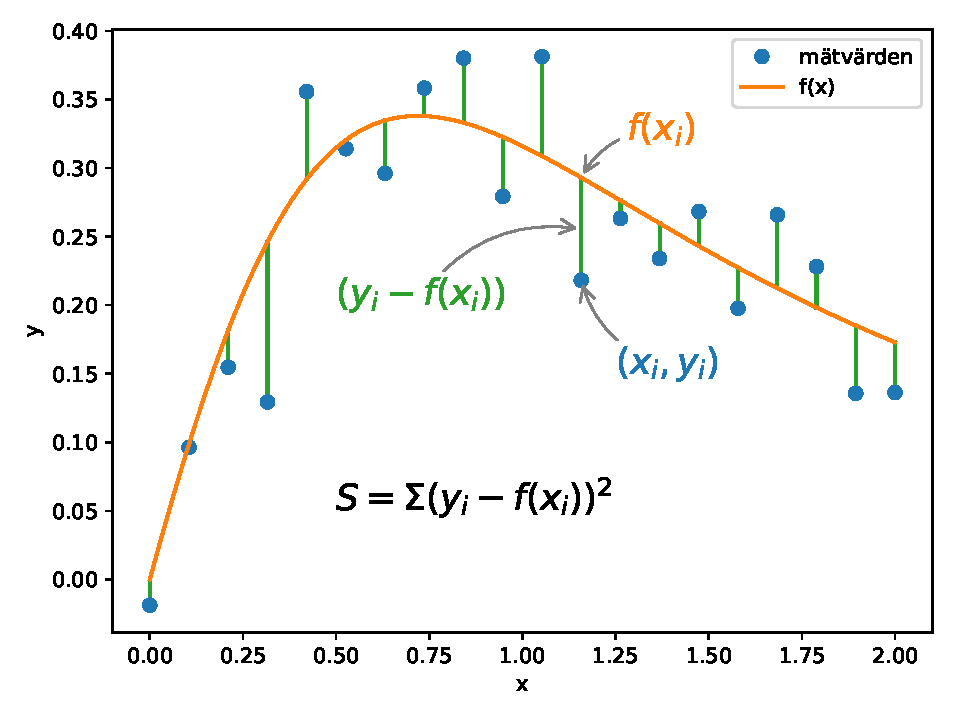
\includegraphics[width=\textwidth]{S.pdf}
        \end{columns}

        \vfill
        Vi kan alltså \emph{minimera} $S$ med avseende på parametrarna $a_j$ för
        att få den bästa anpassningen till vår mätdata! Detta kallas för
        \textcolor{red}{\emph{minstakvadratanpassing}}.

        \begin{equation*}
            \frac{\partial S}{\partial a_1} = 0,
            \frac{\partial S}{\partial a_2} = 0,\quad\ldots,
            \frac{\partial S}{\partial a_m} = 0
        \end{equation*}
        Observera att derivatorna tas med avseende på parametrarna $a_j$ (\textbf{inte} mätvärdena)!
    \end{frame}

    \begin{frame}
        Exempel: Anpassa en linje $y=a_1x + a_2$ till en mätserie $\{x_i, y_i\}$.
        \begin{columns}
            \column{.3\textwidth}
            \begin{table}[]
                \centering
                \begin{tabular}{c|c}
                    $x_i$ & $y_i$   \\ \hline
                    0 & 1.8 \\
                    1 & 2.6 \\
                    2 & 2.1 \\
                    3 & 3.7 \\
                    4 & 3.5 \\
                    5 & 4.5 \\
                    6 & 4.8 \\
                    7 & 5.2 \\
                    8 & 5.1 \\
                    9 & 6.0
                \end{tabular}
            \end{table}
            \column{0.7\textwidth}
            \begin{figure}
                \centering
                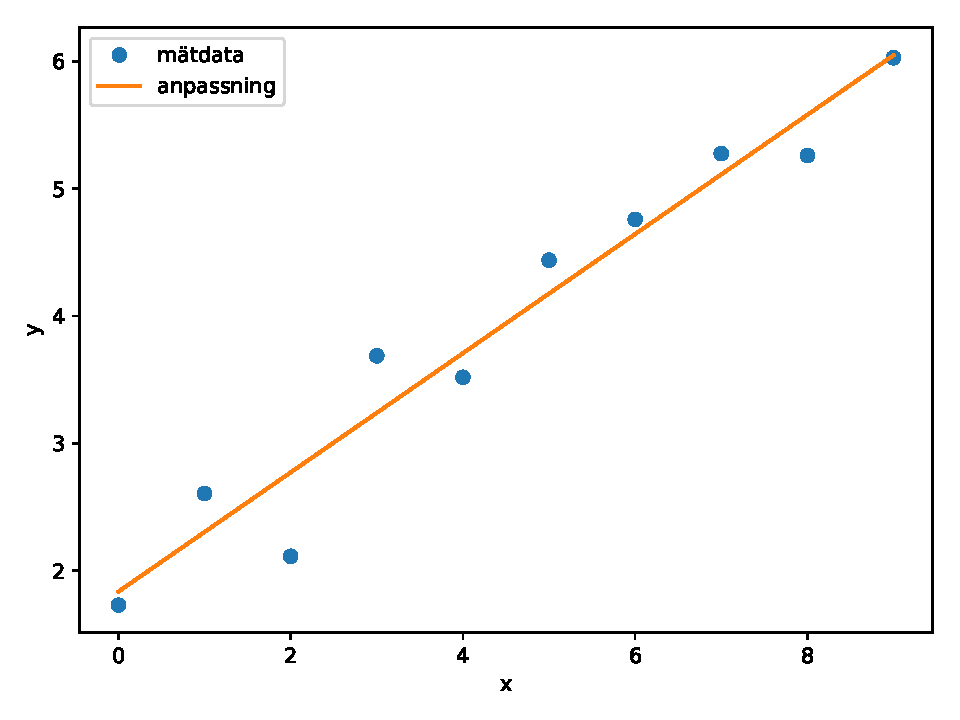
\includegraphics[scale=0.4]{anpassning2.pdf}
            \end{figure}
        \end{columns}
        
        Bilda kvadratsumman $S$:
        \begin{equation*}
            S(a_1, a_2) = \sum_i (y_i - f(x_i,a_1,a_2))^2 = \sum_i (y_i - a_1x_i - a_2)^2
        \end{equation*}
        $S$ är nu en funktion av två variabler, $a_1$ och $a_2$, och måste minimeras över båda!
    \end{frame}
    
    \begin{frame}
        Exempel: Anpassa en linje $y=a_1x + a_2$ till en mätserie $\{x_i, y_i\}$ 
        \begin{columns}[T]
            \column{.5\textwidth}
            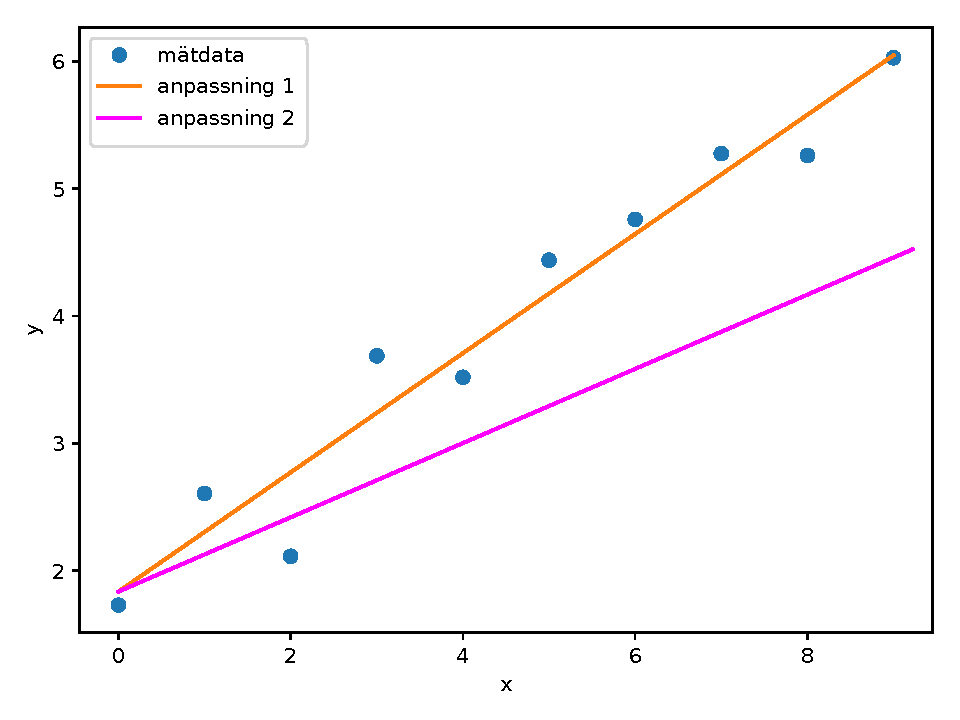
\includegraphics[width=\textwidth]{anpassning2_2.pdf}
            \column{.5\textwidth}
            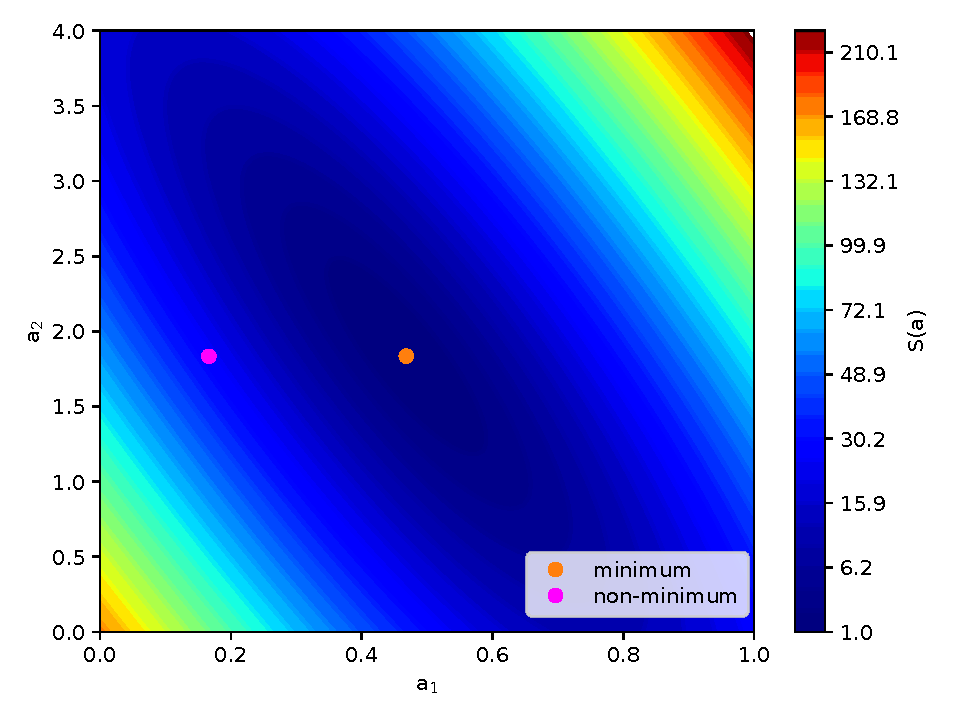
\includegraphics[width=\textwidth]{s2_2.pdf}
        \end{columns}

        Bilda kvadratsumman $S$:
        \begin{equation*}
            S(a_1, a_2) = \sum_i (y_i - f(x_i,a_1,a_2))^2 = \sum_i (y_i - a_1x_i - a_2)^2
        \end{equation*}
        $S$ är nu en funktion av två variabler, $a_1$ och $a_2$, och måste minimeras över båda!
    \end{frame}
    
    
    \begin{frame}
        \onslide<+->
        De partiella derivatorna är då: \null\hfill  \colorbox{gray}{$\left(S = \sum\limits_i\left(y_i - a_1x_i - a_2 \right)^2\right)$}
        \begin{align*}
            \frac{\partial S}{\partial a_1} &= -2\sum_i(y_i - a_1x_i - a_2)x_i = -2\left(\sum_i y_ix_i - \sum_i a_1 x_i^2 - \sum_i a_2 x_i\right) = 0 \\
            \frac{\partial S}{\partial a_2} &= -2\sum_i (y_i - a_1x_i - a_2) = -2\left(\sum_i y_i - \sum_i a_1x_i - \sum_i a_2\right)= 0 \\
        \end{align*}
        \onslide<+->
        Och om vi arrangerar om termerna:
        \begin{align*}
            \sum_i y_ix_i &= a_1 \sum_i x_i^2 + a_2 \sum_i x_i \\% = a_0 \sum_i x_i + a_1\sum_ix_i^2 \\
            \sum_i y_i &= a_1 \sum_i x_i + a_2 \sum_i 1 \\ %= na_0 + a_1\sum_i x_i \\
        \end{align*}
        Detta är ett \emph{linjärt ekvationssystem} i variablerna $a_1$ och $a_2$,
        som kan skrivas om på matrisform (notera $\sum\limits_i 1 = n$):
        \begin{equation*}
            \begin{pmatrix}
                \sum_i y_ix_i \\
                \sum_i y_i
            \end{pmatrix} =
            \begin{pmatrix}
                \sum_i x_i^2 & \sum_ix_i \\
                \sum_i x_i  & n \\
            \end{pmatrix}
            \begin{pmatrix}
                a_1 \\
                a_2
            \end{pmatrix}
        \end{equation*}
    \end{frame}

    \begin{frame}[fragile]
        Om vi sätter
        \begin{equation*}
            \vec h =
            \begin{pmatrix}
                \sum_i y_ix_i \\
                \sum_i y_i
            \end{pmatrix},\quad
            G =
            \begin{pmatrix}
                \sum_i x_i^2 & \sum_ix_i \\
                \sum_i x_i & n
            \end{pmatrix},\quad
            \vec a =
            \begin{pmatrix}
                a_1 \\
                a_2
            \end{pmatrix}
        \end{equation*}
        kan detta skrivas som $G\vec a = \vec h$ och allt vi behöver göra är att lösa för $\vec a$:
        \begin{equation*}
            \vec a = G^{-1}\vec h
        \end{equation*}

        I Matlab:
        \begin{minted}[frame=leftline,framesep=2mm,autogobble,escapeinside=||]{matlab}
            x = [|\ldots|]; y = [|\ldots|]; % mätdata |$\{x_i, y_i\}$|
            G = [sum(x.^2), sum(x); sum(x), length(x)]; % matrisen |$G$|
            h = [sum(y.*x); sum(y)]; % högerledet |$h$|
            a = inv(G)*h % de anpassade parametrarna |$a = (a_1, a_2)^\top$|
        \end{minted}


    \end{frame}

    \begin{frame}[fragile]{Osäkerheterna i $a_1$ och $a_2$}
        Eftersom våra mätvärden $\{x_i, y_i\}$ har en viss spridning finns det
        en osäkerhet i de anpassade parametrarna $\vec a = (a_1,\ldots,a_j,\ldots,a_m)^\top$. Denna ges av
        \begin{equation*}
            u(a_j) = \sqrt{\frac{(G^{-1})_{jj}S}{n - m}}
        \end{equation*}
        där
        \begin{itemize}
            \item $(G^{-1})_{jj}$ är diagonalelementen i $G^{-1}$,
            \item $S=\sum_i(y_i - f(x_i,\vec a))^2$ är kvadratsumman som tidigare,
            \item $n$ är antalet mätpunkter och $m$ är antalet anpassade parametrar.
                \begin{itemize}
                    \item $n-m$ kallas för antalet \emph{frihetsgrader} och betecknas $\nu = n - m$.
                \end{itemize}
        \end{itemize}

        \vfill
        I Matlab:
        \begin{minted}[frame=leftline,framesep=2mm,autogobble,escapeinside=||]{matlab}
            a = inv(G)*h % de anpassade parametrarna |$a = (a_1,\ldots,a_m)^\top$|
            S = sum((y-f(x,a)).^2); % kvadratsumman |$S(a) = \sum(y_i - f(x_i, a))^2$|
            n = length(x); m = length(a); % #mätvärden |$n$| och #parametrar |$m$|

            % vektor med mätosäkerheterna |$u_a = (u_{a_1},\ldots,u_{a_m})^\top$|
            ua = sqrt(diag(inv(G))*S/(n - m));
        \end{minted}
    \end{frame}

    \begin{frame}[fragile]
        Komplett matlab-exempel för vår räta linje:

        \begin{minted}[frame=leftline,framesep=2mm,autogobble,escapeinside=||]{matlab}
            x = [|\ldots|]; y = [|\ldots|]; % mätdata |$\{x_i, y_i\}$|
            G = [sum(x.^2), sum(x); sum(x), length(x)]; % matrisen |$G$|
            h = [sum(y.*x); sum(y)]; % högerledet |$h$|
            a = inv(G)*h % de anpassade parametrarna |$a = (a_1, a_2)^\top$|

            S = sum((y-a(1)*x-a(2)).^2); % kvadratsumman |$S(a) = \sum(y_i - a_1x_i - a_2)^2$|
            n = length(x); m = length(a); % #mätvärden |$n$| och #parametrar |$m$|
            ua = sqrt(diag(inv(G))*S/(n - m)); % mätosäkerheter |$u_a = (u_{a_1},u_{a_2})^\top$|
        \end{minted}

        \vfill
        Detta ger
        \begin{equation*}
            \vec a =
            \begin{pmatrix}
                0.46823 \\
                1.84421
            \end{pmatrix},\quad
            \vec u_a =
            \begin{pmatrix}
                0.03901 \\
                0.21394
            \end{pmatrix}
        \end{equation*}
        dvs
        \begin{align*}
            a_1 &= \num{0.468\pm0.039} \\
            a_2 &= \num{1.84\pm0.21}
        \end{align*}
        (notera att vi avrundat till två värdesiffor i mätosäkerheterna)
    \end{frame}



\end{document}